\documentclass[landscape,a0paper,fontscale=0.285]{baposter}

\usepackage{calc}
\usepackage{graphicx}
\usepackage{amsmath}
\usepackage{amssymb}
\usepackage{relsize}
\usepackage{multirow}
\usepackage{rotating}
\usepackage{bm}
\usepackage{url}

\usepackage{multicol}

%\usepackage{times}
%\usepackage{helvet}
%\usepackage{bookman}
\usepackage{palatino}
%\usepackage{algorithm}
\usepackage{algpseudocode}
\usepackage[linesnumbered, noline, noend]{algorithm2e}

\newcommand{\captionfont}{\footnotesize}

\DeclareGraphicsExtensions{.pdf,.jpg,.png}


\usetikzlibrary{calc}

\newcommand{\SET}[1]  {\ensuremath{\mathcal{#1}}}
\newcommand{\MAT}[1]  {\ensuremath{\boldsymbol{#1}}}
\newcommand{\VEC}[1]  {\ensuremath{\boldsymbol{#1}}}
\newcommand{\Video}{\SET{V}}
\newcommand{\video}{\VEC{f}}
\newcommand{\track}{x}
\newcommand{\Track}{\SET T}
\newcommand{\LMs}{\SET L}
\newcommand{\lm}{l}
\newcommand{\PosE}{\SET P}
\newcommand{\posE}{\VEC p}
\newcommand{\negE}{\VEC n}
\newcommand{\NegE}{\SET N}
\newcommand{\Occluded}{\SET O}
\newcommand{\occluded}{o}

%%%%%%%%%%%%%%%%%%%%%%%%%%%%%%%%%%%%%%%%%%%%%%%%%%%%%%%%%%%%%%%%%%%%%%%%%%%%%%%%
%%%% Some math symbols used in the text
%%%%%%%%%%%%%%%%%%%%%%%%%%%%%%%%%%%%%%%%%%%%%%%%%%%%%%%%%%%%%%%%%%%%%%%%%%%%%%%%

%%%%%%%%%%%%%%%%%%%%%%%%%%%%%%%%%%%%%%%%%%%%%%%%%%%%%%%%%%%%%%%%%%%%%%%%%%%%%%%%
% Multicol Settings
%%%%%%%%%%%%%%%%%%%%%%%%%%%%%%%%%%%%%%%%%%%%%%%%%%%%%%%%%%%%%%%%%%%%%%%%%%%%%%%%
\setlength{\columnsep}{1.5em}
\setlength{\columnseprule}{0mm}

%%%%%%%%%%%%%%%%%%%%%%%%%%%%%%%%%%%%%%%%%%%%%%%%%%%%%%%%%%%%%%%%%%%%%%%%%%%%%%%%
% Save space in lists. Use this after the opening of the list
%%%%%%%%%%%%%%%%%%%%%%%%%%%%%%%%%%%%%%%%%%%%%%%%%%%%%%%%%%%%%%%%%%%%%%%%%%%%%%%%
\newcommand{\compresslist}{%
\setlength{\itemsep}{1pt}%
\setlength{\parskip}{0pt}%
\setlength{\parsep}{0pt}%
}

\newcommand*{\one} {\mathbf{1}}
\newcommand{\indicator}[1]{ \one \{ #1 \} }
\DeclareMathOperator*{\argmin}{arg\,min}
\DeclareMathOperator*{\argmax}{arg\,max}
%%%%%%%%%%%%%%%%%%%%%%%%%%%%%%%%%%%%%%%%%%%%%%%%%%%%%%%%%%%%%%%%%%%%%%%%%%%%%%
%%% Begin of Document
%%%%%%%%%%%%%%%%%%%%%%%%%%%%%%%%%%%%%%%%%%%%%%%%%%%%%%%%%%%%%%%%%%%%%%%%%%%%%%

\begin{document}

%%%%%%%%%%%%%%%%%%%%%%%%%%%%%%%%%%%%%%%%%%%%%%%%%%%%%%%%%%%%%%%%%%%%%%%%%%%%%%
%%% Here starts the poster
%%%---------------------------------------------------------------------------
%%% Format it to your taste with the options
%%%%%%%%%%%%%%%%%%%%%%%%%%%%%%%%%%%%%%%%%%%%%%%%%%%%%%%%%%%%%%%%%%%%%%%%%%%%%%
% Define some colors

%\definecolor{lightblue}{cmyk}{0.83,0.24,0,0.12}
\definecolor{lightblue}{rgb}{0.145,0.6666,1}

\hyphenation{resolution occlusions}
%%
\begin{poster}%
  % Poster Options
  {
  % Show grid to help with alignment
  grid=false,
  % Column spacing
  colspacing=1em,
  % Color style
  bgColorOne=white,
  bgColorTwo=white,
  borderColor=lightblue,
  headerColorOne=black,
  headerColorTwo=lightblue,
  headerFontColor=white,
  boxColorOne=white,
  boxColorTwo=lightblue,
  % Format of textbox
  textborder=roundedleft,
  % Format of text header
  eyecatcher=true,
  headerborder=closed,
  headerheight=0.1\textheight,
%  textfont=\sc, An example of changing the text font
  headershape=roundedright,
  headershade=shadelr,
  headerfont=\Large\bf\textsc, %Sans Serif
  textfont={\setlength{\parindent}{1.5em}},
  boxshade=plain,
%  background=shade-tb,
  background=plain,
  linewidth=2pt
  }
  % Eye Catcher
  {
\includegraphics[height=5em]{SU_New_BlockStree_2color}}
  % Title
  {\bf\textsc{Learn to play Go}\vspace{0.5em}}
  % Authors
  {\textsc{Albert Liu (albertpl@stanford.edu})}
  % University logo
  {% The makebox allows the title to flow into the logo, this is a hack because of the L shaped logo.
    
\includegraphics[height=5.0em]{SU_Seal_Red}
  }

%%%%%%%%%%%%%%%%%%%%%%%%%%%%%%%%%%%%%%%%%%%%%%%%%%%%%%%%%%%%%%%%%%%%%%%%%%%%%%
%%% Now define the boxes that make up the poster
%%%---------------------------------------------------------------------------
%%% Each box has a name and can be placed absolutely or relatively.
%%% The only inconvenience is that you can only specify a relative position
%%% towards an already declared box. So if you have a box attached to the
%%% bottom, one to the top and a third one which should be in between, you
%%% have to specify the top and bottom boxes before you specify the middle
%%% box.
%%%%%%%%%%%%%%%%%%%%%%%%%%%%%%%%%%%%%%%%%%%%%%%%%%%%%%%%%%%%%%%%%%%%%%%%%%%%%%
    %
    % A coloured circle useful as a bullet with an adjustably strong filling
    \newcommand{\colouredcircle}{%
      \tikz{\useasboundingbox (-0.2em,-0.32em) rectangle(0.2em,0.32em);
            \draw[draw=black,fill=lightblue,line width=0.03em] (0,0) circle(0.18em);
      }
    }


%%%%%%%%%%%%%%%%%%%%%%%%%%%%%%%%%%%%%%%%%%%%%%%%%%%%%%%%%%%%%%%%%%%%%%%%%%%%%%
 \headerbox{Motivation \& Challenges}{name=motivation,column=0, row=0}{
%%%%%%%%%%%%%%%%%%%%%%%%%%%%%%%%%%%%%%%%%%%%%%%%%%%%%%%%%%%%%%%%%%%%%%%%%%%%%%
\centering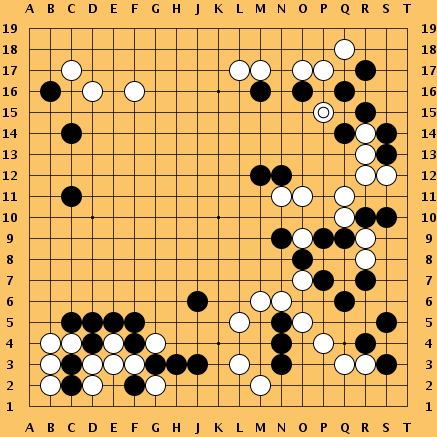
\includegraphics[width=0.6\linewidth]{goboard}


\begin{itemize}
  \item
    simple rules but mastering requires many years of study by human
  \item
    considered hardest classic board game and grand challenge for AI
  \item
    AlphaGo and AlphaGoZero have rocked the Go and AI world

\item
  Challenges
  \begin{itemize}
    \item
    state based search is intractable due enormous search space $(\sim 10^{170})$, large number of legal move per state$(\sim 250)$
    \item
    massive computational requirements for MCTS and training DNN
  \item
    lack of domain expertise
    
  \end{itemize}
  \vspace{1.0em}
\end{itemize}

}


%%%%%%%%%%%%%%%%%%%%%%%%%%%%%%%%%%%%%%%%%%%%%%%%%%%%%%%%%%%%%%%%%%%%%%%%%%%%%%
    \headerbox{Problem Definition}{name=problem,column=0,below=motivation, above=bottom}{
%%%%%%%%%%%%%%%%%%%%%%%%%%%%%%%%%%%%%%%%%%%%%%%%%%%%%%%%%%%%%%%%%%%%%%%%%%%%%%
\begin{itemize} 
  \item
  Pachi built-in \textit{UCT} engine as our oracle which is said to achieve highest amateur expect level (KGS 7 dan) on $9 \times 9$ board.  
  \item
  To learn playing Go  without incorporating lots of heuristics and predefined patterns beyond basic Go rules
  \item
    To understand pro and con of various approaches.
\end{itemize}


%\centering\includegraphics[width=0.98\linewidth]{problem}

 }

%%%%%%%%%%%%%%%%%%%%%%%%%%%%%%%%%%%%%%%%%%%%%%%%%%%%%%%%%%%%%%%%%%%%%%%%%%%%%%
\headerbox{System architecture}{name=design,column=1,span=2,row=0}{
  %%%%%%%%%%%%%%%%%%%%%%%%%%%%%%%%%%%%%%%%%%%%%%%%%%%%%%%%%%%%%%%%%%%%%%%%%%%%%%
\centering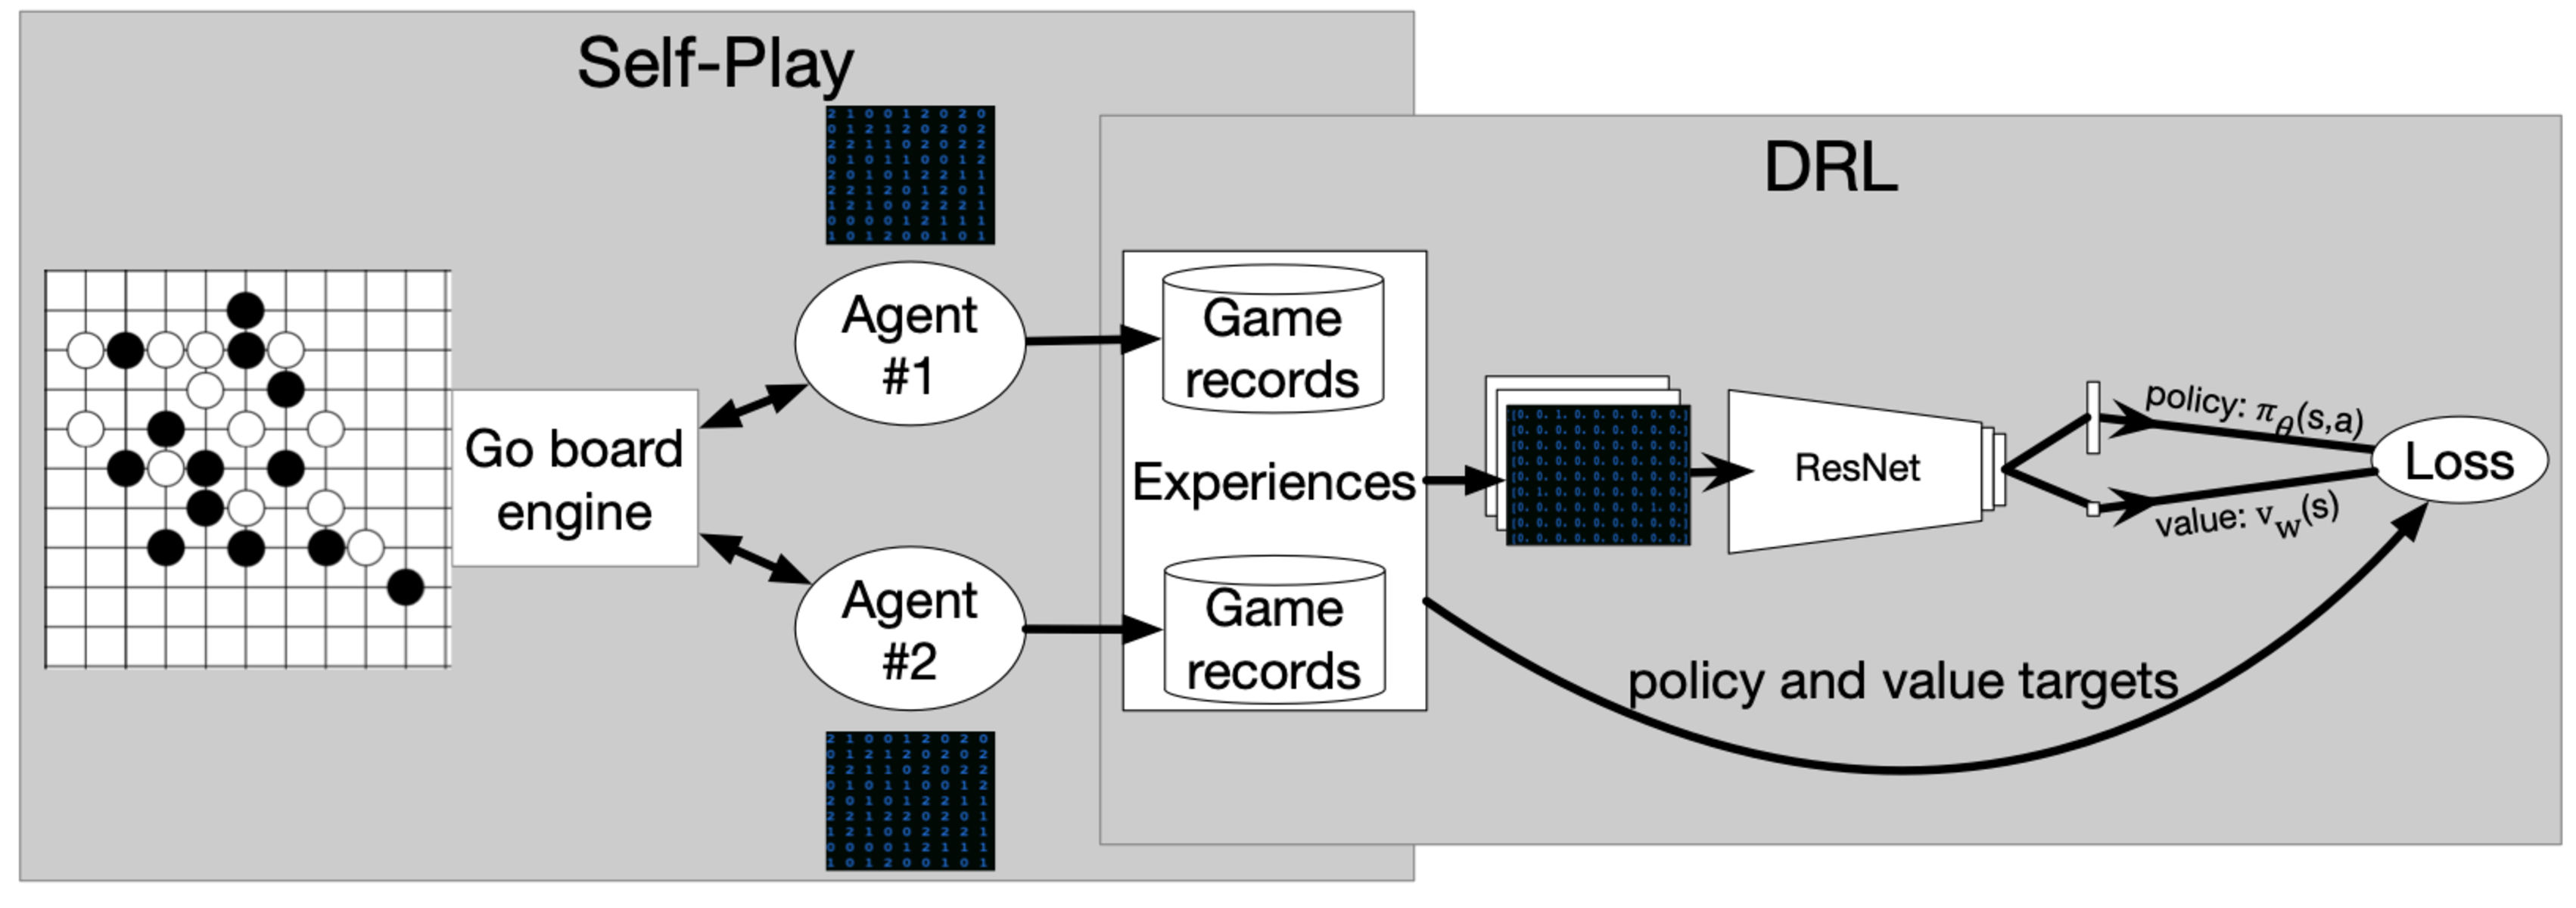
\includegraphics[width=0.98\linewidth]{architecture}
    \begin{itemize} \compresslist
      \item $\pi_{\theta} (A_t|S_t)$
            A probability vector for taking each action $A_t$ for $S_t$.
          \item $v_w(S_t) \in [-1, +1]$
    \end{itemize}

}

%%%%%%%%%%%%%%%%%%%%%%%%%%%%%%%%%%%%%%%%%%%%%%%%%%%%%%%%%%%%%%%%%%%%%%%%%%%%%%
\headerbox{\small{Monte Carlo Tree Search}}{name=mcts,column=1,span=1, below=design, above=bottom}{
%%%%%%%%%%%%%%%%%%%%%%%%%%%%%%%%%%%%%%%%%%%%%%%%%%%%%%%%%%%%%%%%%%%%%%%%%%%%%%
\centering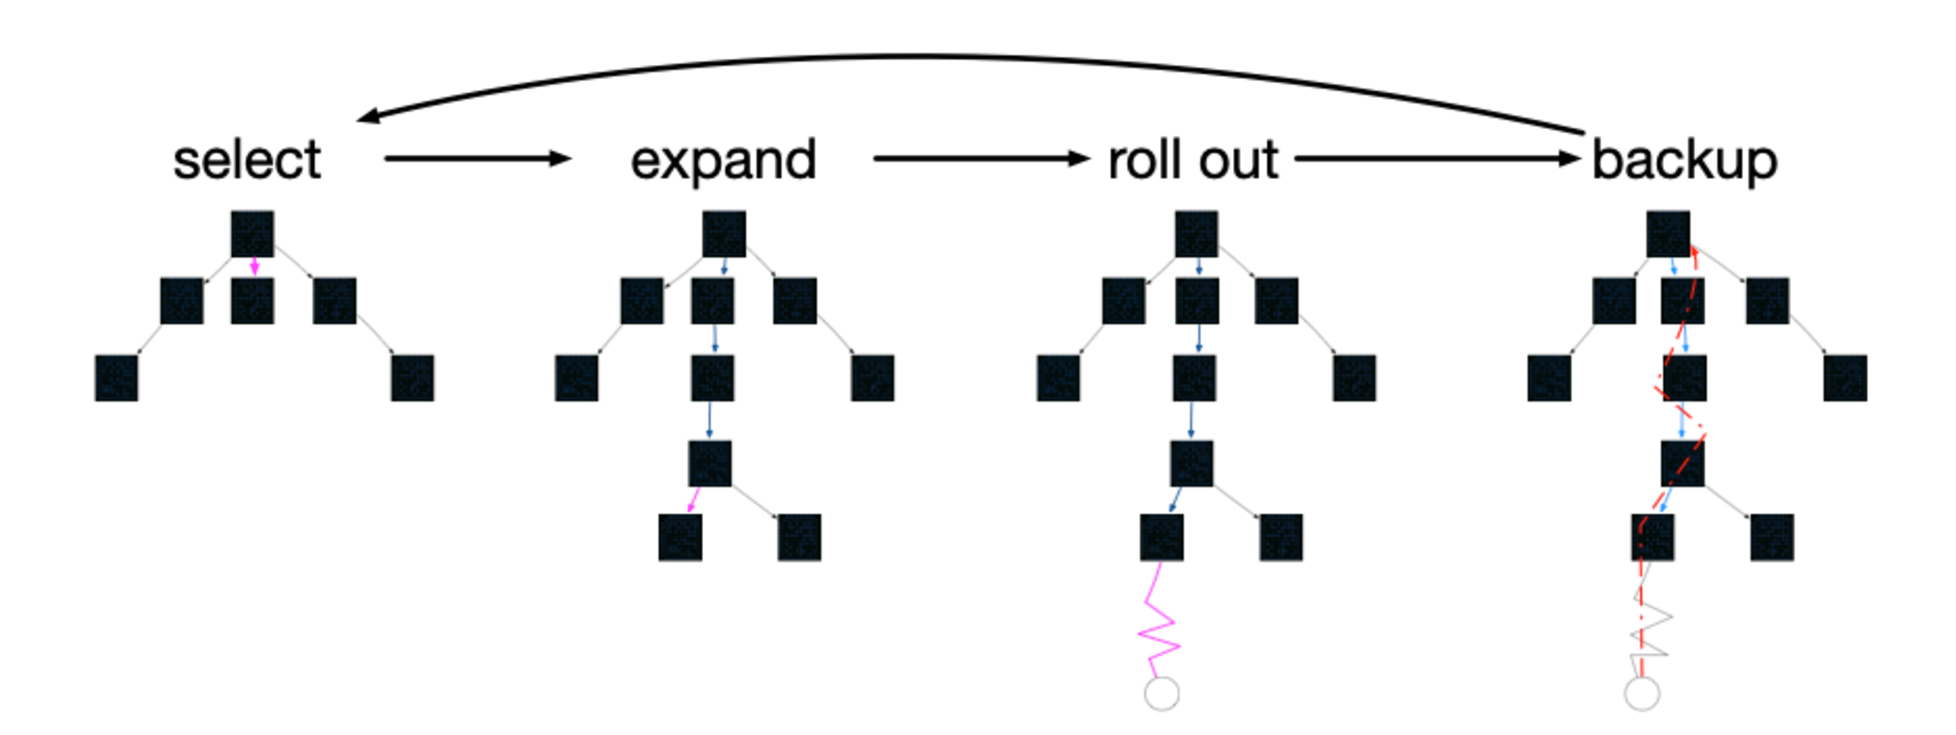
\includegraphics[width=1.0\linewidth]{mcts}


\begin{itemize} \compresslist
  \item Tree policy: UCB1
    $$a  \gets \argmax_{a} q(s, a) + c \sqrt{\frac{\log \sum_{a'}n(s, a')}{n(s,a)}} $$
    Select best within tree.

  \item Rollout policy: random

    Sampling breaks curse of dimensionality

  \end{itemize}

\centering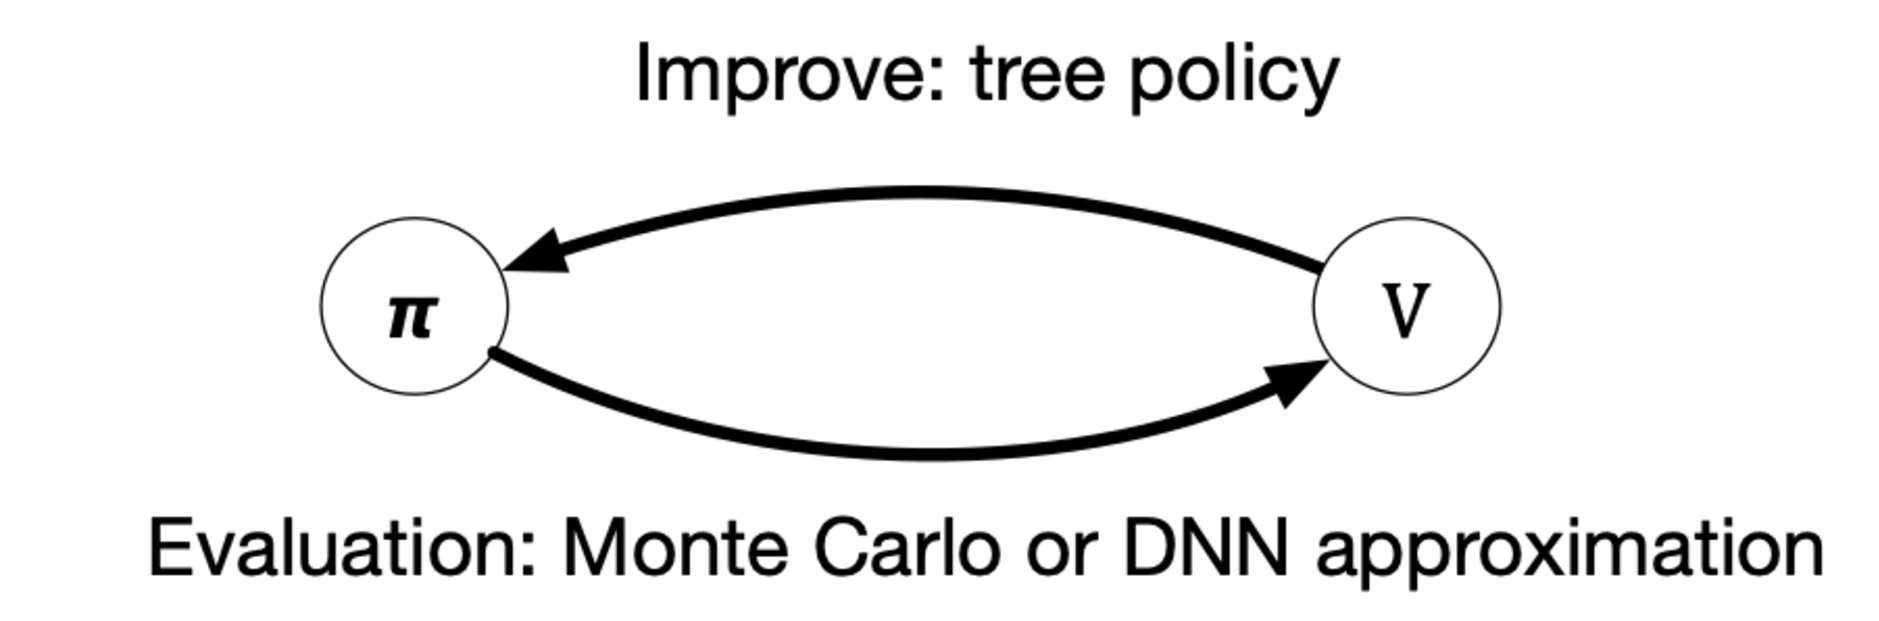
\includegraphics[width=1.0\linewidth]{gpi}

}


%%%%%%%%%%%%%%%%%%%%%%%%%%%%%%%%%%%%%%%%%%%%%%%%%%%%%%%%%%%%%%%%%%%%%%%%%%%%%%
  \headerbox{\small Deep Reinforcement Learning}{name=rl,column=2, span=1, below=design, above=bottom}{
%%%%%%%%%%%%%%%%%%%%%%%%%%%%%%%%%%%%%%%%%%%%%%%%%%%%%%%%%%%%%%%%%%%%%%%%%%%%%%
    \begin{itemize} \compresslist
      \item REINFORCE with Baseline

        $\pi_{\theta}(s,a)$ to approximate police. $v_w(s)$ as baseline to reduce variance.
\begin{align*}
\theta_{t+1} 
& \gets 
\theta_{t} + \alpha 
( r_t  - v_w(s_t))
\nabla_{\theta} \log \pi_{\theta}(a_t|s_t) 
\\
w_{t+1} 
&\gets 
w_{t} + \alpha 
( r  - v_w(s_t))
\nabla_{w} v_w(s_t) 
\end{align*}

      \item Actor-critic with Baseline

        TD error as approximation of advantage.
$$
\scriptstyle
\theta_{t+1} 
\gets 
\theta_{t} + \alpha 
( r + v_w(s_{t+1}) - v_w(s_t))
\nabla_{\theta} \log \pi_{\theta}(a_t|s_t) 
$$

      \item combining DNN and MCTS 


        \begin{itemize} \compresslist
          \item $\pi_{\theta}(s,a)$ as priors for expansion 
          \item $v_w(s)$ as estimated value, no rollout 
          \item supervised training, i.e. as close as possible to statistics from tree search. 
        \end{itemize}
    \end{itemize}

$$a  \gets \argmax_{a} q(s, a) + c \pi_{\theta}(s, a) \frac{\sqrt{\sum_{a'}n(s, a')}}{n(s,a)+1} $$

$$ 
\text{l}(\theta, w) = 
\sum_{i} (v_w(s_t) - r_t)^2 - 
\frac{\sum_{a} n(s_t, a) \log \pi_{\theta}(s_t, a)}
{\sum_{a'} n(s_t, a')}
$$

}


%%%%%%%%%%%%%%%%%%%%%%%%%%%%%%%%%%%%%%%%%%%%%%%%%%%%%%%%%%%%%%%%%%%%%%%%%%%%%%
\headerbox{Preliminary Results}{name=results,column=3,row=0}{
%%%%%%%%%%%%%%%%%%%%%%%%%%%%%%%%%%%%%%%%%%%%%%%%%%%%%%%%%%%%%%%%%%%%%%%%%%%%%%
  All results are averaged over 1000 games of $9 \times 9$ board.


  \begin{itemize} \compresslist
    \item MCTS

  \begin{tabular}{c | c | c | c }
     & random & random & oracle  \\
    \hline
    rollouts  & 100 & 1000 & 1000 \\
    win rate  & 0.92 & 0.99 & 0.16 \\
    time & 2.4 & 29.3 & 35.1 \\ 
  \end{tabular}

  \item REINFORCE with baseline v.s. oracle

  \begin{tabular}{c | c  }
     iteration &   win rate\\
    \hline
    1  & 0.025  \\
    2 & 0.0265  \\
    3 & 0.0375  \\ 
    4 & 0.055  \\ 
  \end{tabular}
  \end{itemize}

  \vspace{0.5em}
}


%%%%%%%%%%%%%%%%%%%%%%%%%%%%%%%%%%%%%%%%%%%%%%%%%%%%%%%%%%%%%%%%%%%%%%%%%%%%%%
\headerbox{Analysis}{name=analysis,column=3,span=1, below=results, above=bottom}{
  %%%%%%%%%%%%%%%%%%%%%%%%%%%%%%%%%%%%%%%%%%%%%%%%%%%%%%%%%%%%%%%%%%%%%%%%%%%%%%
\begin{itemize} \compresslist
  \item MCTS
    pachi uses \textbf{heavy} rollout policy, which entails rule based pattern, such as,  if the last move has put its own group in \textit{atari} we capture it; \textit{Nakade}a move is played inside the eyeshape to prevent the opponent from splitting it into two eyes.  Also Pachi applies heuristics based priors when expanding new node. 

  \item
    Our MCTS uses random rollout policy and not as strong as it could be.

  \item
    Self-played based DRL approaches require 


\end{itemize}
}


\end{poster}

\end{document}
